%!TEX root = ../my_thesis.tex
\chapter{Conception d'un processeur par la définition de son architecture} % (fold)
\label{chap:tta}

Une nouvelle méthodologie est employée afin de définir une architecture de processeur efficace pour le décodage de codes polaires. Elle fait partie de la famille des architectures TTA.

La section~\ref{sec:tta_description} de ce chapitre présente la structure générale et les propriétés des processeurs TTA. Une des caractéristiques principales de ces architectures est leur haut degré de parallélisme. Les processeurs TTA se rapprochent des architectures VLIW. Celles-ci sont donc introduites afin de servir de point de comparaison. Un exemple d'architecture TTA est ensuite donné afin d'en illustrer son fonctionnement. La suite logicielle libre utilisée pour concevoir le processeur est nommée TCE. Ces outils permettent l'automatisation d'une grande partie de la conception des processeurs TTA. La seconde partie de la section illustre et décrit le flot de conception et le rôle des différents outils. La section~\ref{sec:tta_design} détaille la conception de deux processeurs TTA à haute performance pour le décodage de codes polaires. La première architecture supporte l'algorithme SC et la seconde supporte à la fois les algorithmes SC et SCAN. Les expérimentations et les mesures réalisées sont présentées dans la section~\ref{sec:tta_res}.

\vspace*{\fill}
\minitocTITI
\vspace*{\fill}
\newpage

\section{Transport Triggered Architectures}
\label{sec:tta_description}

\subsection{Principes et caractéristiques des processeurs TTA}

Dans le chapitre précédent, l'architecture d'un processeur RISC a été modifiée et son jeu d'instructions étendu afin d'obtenir un ASIP dédié au décodage des codes polaires. Dans ce chapitre, une approche différente est envisagée, qui consiste à définir un processeur de type TTA (Transport Triggered Architecture).
Les architectures de type TTA se rapprochent des architectures à très long mot d'instructions (VLIW : Very Long Instruction Word) avec néanmoins une plus grande modularité. Il est ainsi possible de rajouter des unités fonctionnelles personnalisées et de définir précisément la manière dont celles-ci sont interconnectées. Le concepteur de l'architecture est amené à sélectionner chaque unité matérielle et à spécifier précisément leur modèle matériel. La structure et les performances de l'architecture obtenue se rapprochent de celles des architectures matérielles dédiées tout en conservant la programmabilité d'un processeur généraliste. En effet, les fonctionnalités d'un processeur généraliste sont conservées. De plus, les architectures TTA bénéficient d'un écosystème d'outils qui facilitent la conception et le développement de ce type de processeurs. Le programme devant s'exécuter sur l'architecture est décrit à l'aide d'un langage de programmation haut niveau  (C, C++, OpenCL). Des outils de profilage et de débogage sont disponibles et une grande partie du modèle matériel est généré automatiquement. Dans ce chapitre, nous proposons donc une architecture de type TTA pour le décodage de codes polaires.

Dans une architecture de processeur, nous distinguons habituellement deux types de parallélisme.
Le premier est le parallélisme de données.
Pour exploiter ce parallélisme, les jeux d'instructions de certains processeurs incluent des instructions vectorielles SIMD.
C'est le cas des architectures ARM ou x86 actuelles qui implémentent respectivement les jeux d'instructions NEON et AVX utilisés dans le chapitre~\ref{chap:soft_scl}.
Les instructions spécialisées de l'ASIP proposé dans le chapitre~\ref{chap:tensilica} sont également des instructions SIMD.
Ces instructions permettent d'appliquer parallèlement une même opération sur plusieurs données.

Le second type de parallélisme est le parallélisme d'instructions. Contrairement au parallélisme de données, il s'agit d'exécuter des opérations différentes sur plusieurs données d'entrées. Par exemple, effectuer une somme de deux données et, en parallèle, effectuer une opération \textit{ou-exclusif} sur deux autres.
Il existe plusieurs façons de concevoir un processeur permettant du parallélisme d'instructions. Le compilateur peut selon les cas être impliqué dans la détection et l'exploitation du parallélisme d'instructions.

Dans les architectures superscalaires, le compilateur n'est pas impliqué dans la gestion du parallélisme d'instructions. Celui-ci est détecté par des unités matérielles spécialisées. 
Elles permettent de lancer l'exécution en parallèle de plusieurs opérations indépendantes sur les multiples unités fonctionnelles du processeur.
Pour cela, les unités ont la capacité d'analyser les dépendances entre les données, de changer dynamiquement l'ordre d'exécution des instructions, ainsi que de spéculer sur les futures instructions du programme à exécuter.
Un des avantages de ce type de processeurs est que des programmes séquentiels d'architectures plus anciennes peuvent être accélérés sans nouvelle compilation. Le principal désavantage est une  complexité accrue au niveau de l'architecture processeur causée par l'ajout des unités matérielles en charge de la mise en œuvre du parallélisme. Enfin, la surface du circuit résultant augmente, ainsi que sa consommation énergétique~\cite{rau1993instruction}.

Au contraire, dans les architectures VLIW, l'essentiel de l'effort nécessaire à la mise en œuvre du parallélisme d'instructions est pris en charge par le compilateur. Le compilateur décrit quelles instructions doivent être exécutées en parallèle, et dans quel ordre. L'avantage des architectures VLIW par rapport aux architectures superscalaires est la réduction de la complexité de la logique de contrôle. De plus, les possibilités de parallélisme d'instructions sont plus faciles à identifier par les compilateurs qui ont une vision plus large du programme que les unités matérielles des architectures superscalaires.


\begin{figure}[htp]
\centering
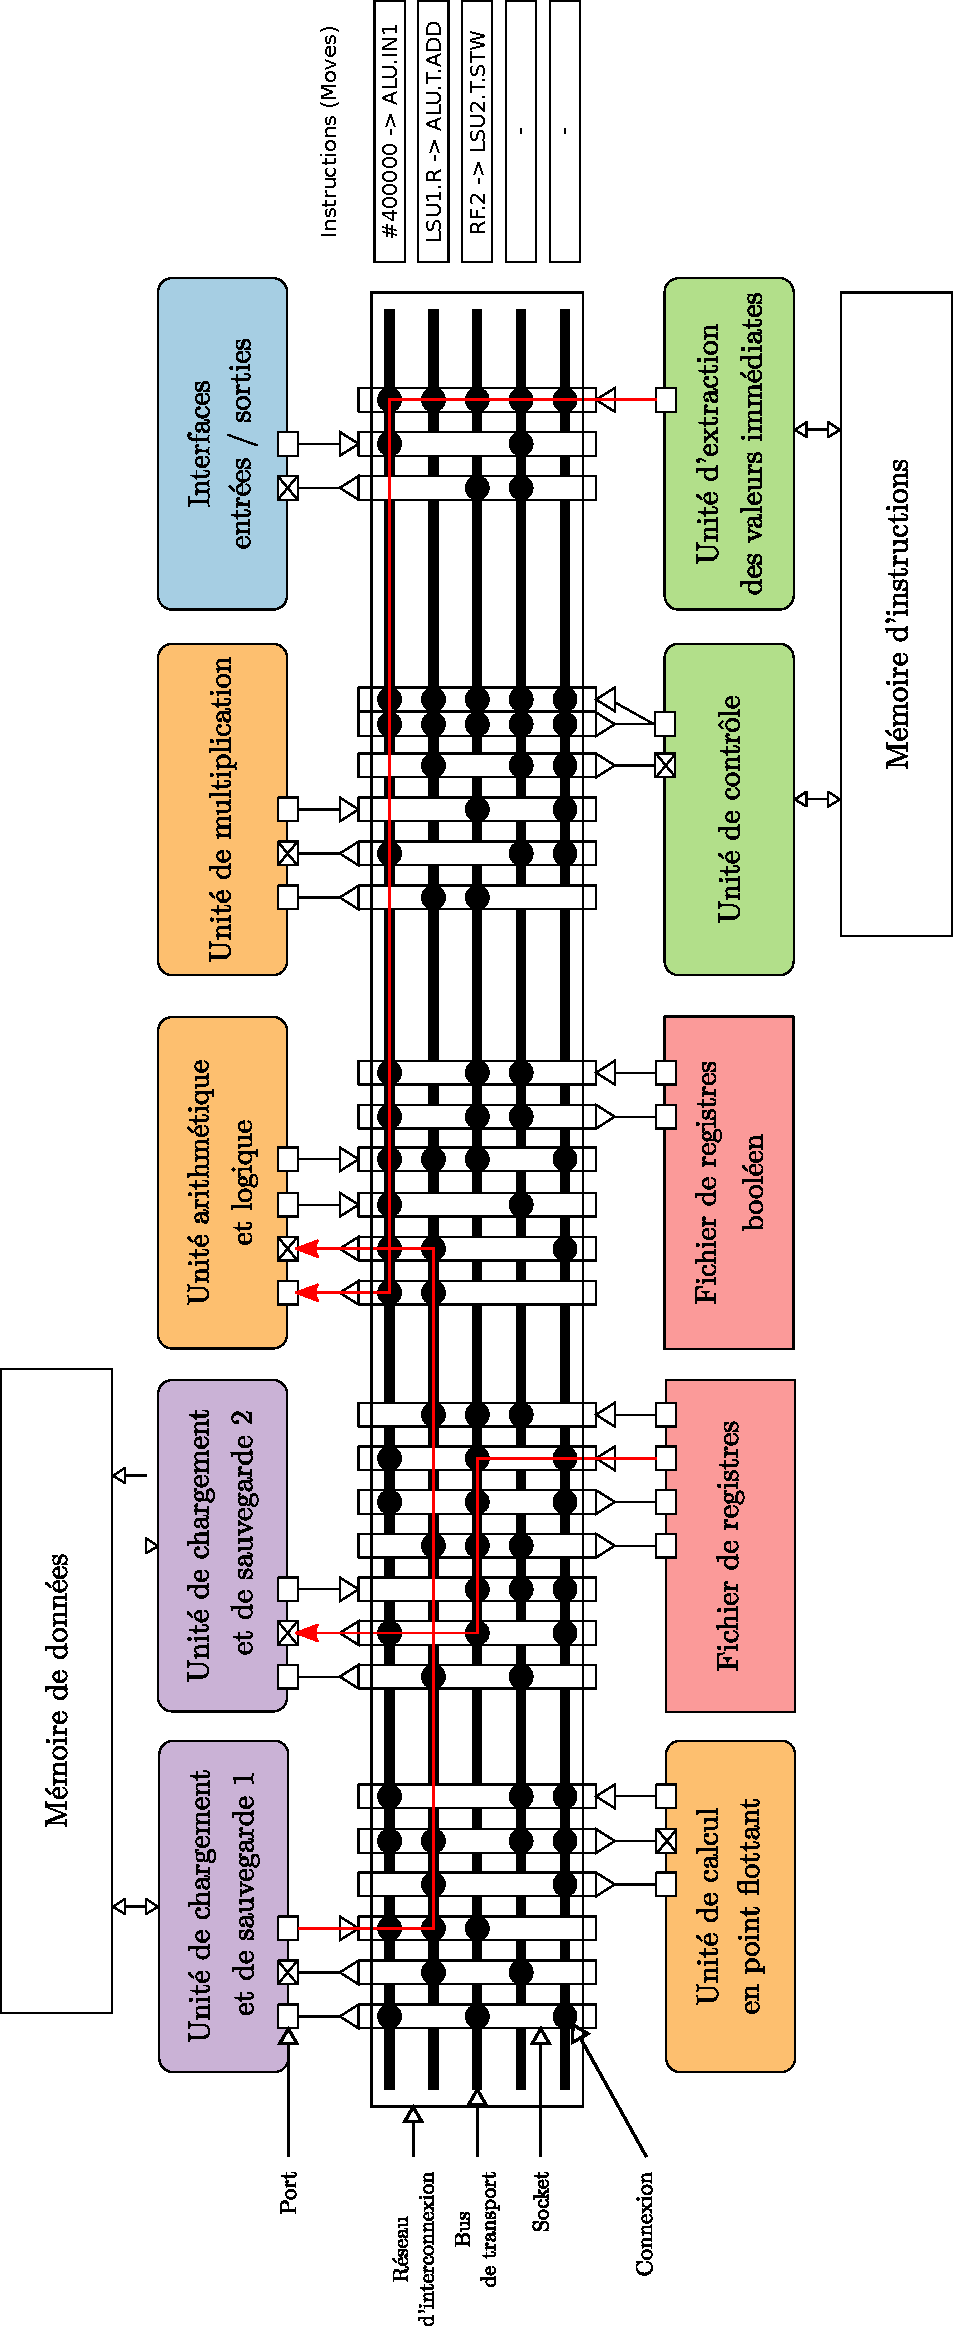
\includegraphics[width=\textwidth]{main/ch4_fig/archi_tta}
\caption{Schéma illustrant les architectures de processeur TTA.}
\label{fig:tta_example}
\end{figure}



L'architecture de processeur proposée dans ce chapitre fait partie de la famille des architectures déclenchées par le transport (TTA : Transport Triggered Architecture). Les TTA sont des architectures modulaires particulières et proches des architectures VLIW~\cite{corporaal_microprocessor_1997}. Les TTAs sont inspirées des architectures MOVE~\cite{1051344}. La Figure~\ref{fig:tta_example} présente un exemple d'architecture TTA~\cite{pekka_phd_2012}. Au centre, nous trouvons les \textit{bus de transport} sur lesquels les données transitent. \`A ces bus de transport sont connectées les \textit{unités fonctionnelles}, par l'intermédiaire de \textit{sockets} et de \textit{ports}. Les \textit{ports} font partie des \textit{unités fonctionnelles} : ils correspondent à des interfaces avec le monde extérieur. Une \textit{socket} est associée à chaque port. Elle n'est pas forcément connectée à tous les bus de transport. Lors de la définition du processeur, c'est au concepteur de décider quels \textit{bus de transport} doivent être connectés à une \textit{socket}. Le nombre de \textit{connexions} doit être soigneusement dimensionné afin de limiter la complexité du \textit{réseau d'interconnexion}.

La différence principale séparant les architectures VLIW classiques et les architectures TTA sont les instructions utilisées. Dans les architectures VLIW, les instructions correspondent aux opérations à effectuer durant chaque cycle d'instruction. Des registres d'entrée et de sortie peuvent être spécifiés selon le type d'instruction. En revanche, un programme exécuté par un processeur d'architecture TTA contient une séquence de transports de données, depuis un port d'une unité fonctionnelle vers un autre. Les opérations sont exécutées lorsqu'une donnée est transmise vers un port particulier d'une unité fonctionnelle, nommé \textit{port de déclenchement}. Chaque unité fonctionnelle possède un seul port de déclenchement.

Dans le schéma de la Figure~\ref{fig:tta_example}, trois transports sont effectués sur les trois bus de gauche (flèches rouges), tandis que les deux bus de droite sont inutilisés. Les instructions correspondantes sont spécifiées au dessus du réseau d'interconnexion (\texttt{\#400000 -> ALU.1}, \texttt{LSU1.3 -> ALU.T.ADD}, \texttt{RF.3 -> LSU2.T.STW}). Le langage utilisé pour décrire les transports est le langage assembleur des architectures TTA, proche du contenu du programme compilé. Dans une instruction TTA, deux ports sont définis : le premier est la source et le second est la destination. Le port est quant à lui spécifié par le nom de son unité fonctionnelle et un identifiant. Lorsque le port de destination est un port de déclenchement (T : Trigger), l'opération déclenchée est également spécifiée. Par exemple, le deuxième transport a pour cible le port de déclenchement de l'unité arithmétique et logique (ALU : Arithmetical and Logical Unit). Il est nécessaire de préciser que l'opération d'addition (ADD) doit être déclenchée : \texttt{ALU.T.ADD}.

Augmenter le nombre d'unités fonctionnelles d'une architecture VLIW est problématique car il est nécessaire d'augmenter le nombre de ports d'écritures et de lecture des files de registres afin que les unités fonctionnelles puissent y accéder simultanément. Ceci a pour conséquence une augmentation de la complexité des files de registre et une possible augmentation du chemin critique.
La modularité des architectures TTA résout ce problème.

En effet, le réseau d'interconnexion et les chemins de données disponibles sont connus du programmeur et du compilateur. Nous parlons de \og chemin de données exposé \fg (\textit{exposed datapath}). Comme le programmeur définit la séquence des transports, et non la séquence des opérations à exécuter, il n'est pas nécessaire de dimensionner les ports des files de registre par rapport au pire cas du nombre d'unités fonctionnelles pouvant accéder simultanément à une file de registres. Le programmeur ne peut qu'affecter des transports de données à des bus disponibles.

De plus, dans les architectures VLIW, les mécanismes de dérivation des registres (\textit{register bypass}) sont implémentés matériellement. Dans les architectures TTA, ils sont décrits par le programmeur. Cela permet de réduire l'engorgement des registres et donc la nécessité de ports supplémentaires sur chaque file de registres.

Ces différentes caractéristiques ont guidé notre choix dans la sélection des architectures TTA pour la conception d'architectures programmables de décodage de codes polaires. Elles résolvent en effet le problème identifié en conclusion du chapitre~\ref{chap:tensilica}, à savoir le nombre d'échanges nécessaires entre les mémoires, les files de registres et les unités fonctionnelles. La modularité des architectures TTA doit nous permettre de définir finement un réseau d'interconnexion permettant des communications directes entre les mémoires et les unités fonctionnelles, mais également entre les unités fonctionnelles elles-même.

Une autre raison justifiant ce choix est la disponibilité d'une suite logicielle libre et mature nommée TCE permettant une conception efficace d'architectures TTA. La suite logicielle offre également un compilateur adaptatif qui permet l'écriture des programmes dans des langages de haut niveau (C / C++). De plus, un contact a été établi avec l'équipe à l'origine de cette suite logicielle, qui nous a apporté un soutien technique efficace au long du développement. Cette suite logicielle est décrite dans la sous-section suivante.


\subsection{L'environnement TCE}

\subsubsection{Définition de l'architecture et de l'implémentation du processeur}

L'environnement TCE (TTA-based Co-design Environment) est une suite d'outils logiciels permettant la description d'architectures TTA, la compilation de programmes exécutables sur ces architectures et la génération de modèles matériels synthétisables et implémentables~\cite{jaaskelainen_hw/sw_2017}. Une version améliorée de l'outil, nommée TCEMC (TCE MultiCore), permet le support d'opérations SIMD~\cite{tcemc_2011}. Nous l'avons utilisée pour concevoir les décodeurs polaires. La Figure~\ref{fig:tce} présente l'ensemble des outils proposés, les fichiers intermédiaires générés et le flot de conception.

Le premier outil utilisé est l'éditeur de modèle architectural (\textbf{prode}). Il s'agit d'une interface graphique qui facilite la définition de processeurs tels que celui présenté dans la Figure~\ref{fig:tta_example}. Le fichier \textit{.adf} contient le nombre de bus et la largeur de chaque bus, la liste des sockets et de leurs connexions avec les bus de transport et les ports des unités fonctionnelles. Ce fichier liste également les unités fonctionnelles.

Le fichier \textit{.adf} récapitule également les opérations que chaque unité fonctionnelle est capable de réaliser. Chaque opération est décrite par son interface, contenue dans un fichier \textit{.opp} et son comportement, défini par un fichier \textit{.c} ou \textit{.cpp}. L'éditeur de la base de données des opérations (\textbf{osed}) permet d'explorer et d'éditer les différentes opérations. Il est également en charge de compiler les modèles comportementaux. L'exécutable (\textit{.opb}) est utilisé pour effectuer des simulations de l'opération, soit de manière individuelle, soit au sein du simulateur du programme complet. L'outil \textit{prode}, quant à lui, associe les unités fonctionnelles aux opérations dans le fichier \textit{.adf}.

\begin{figure}[htp]
\centering
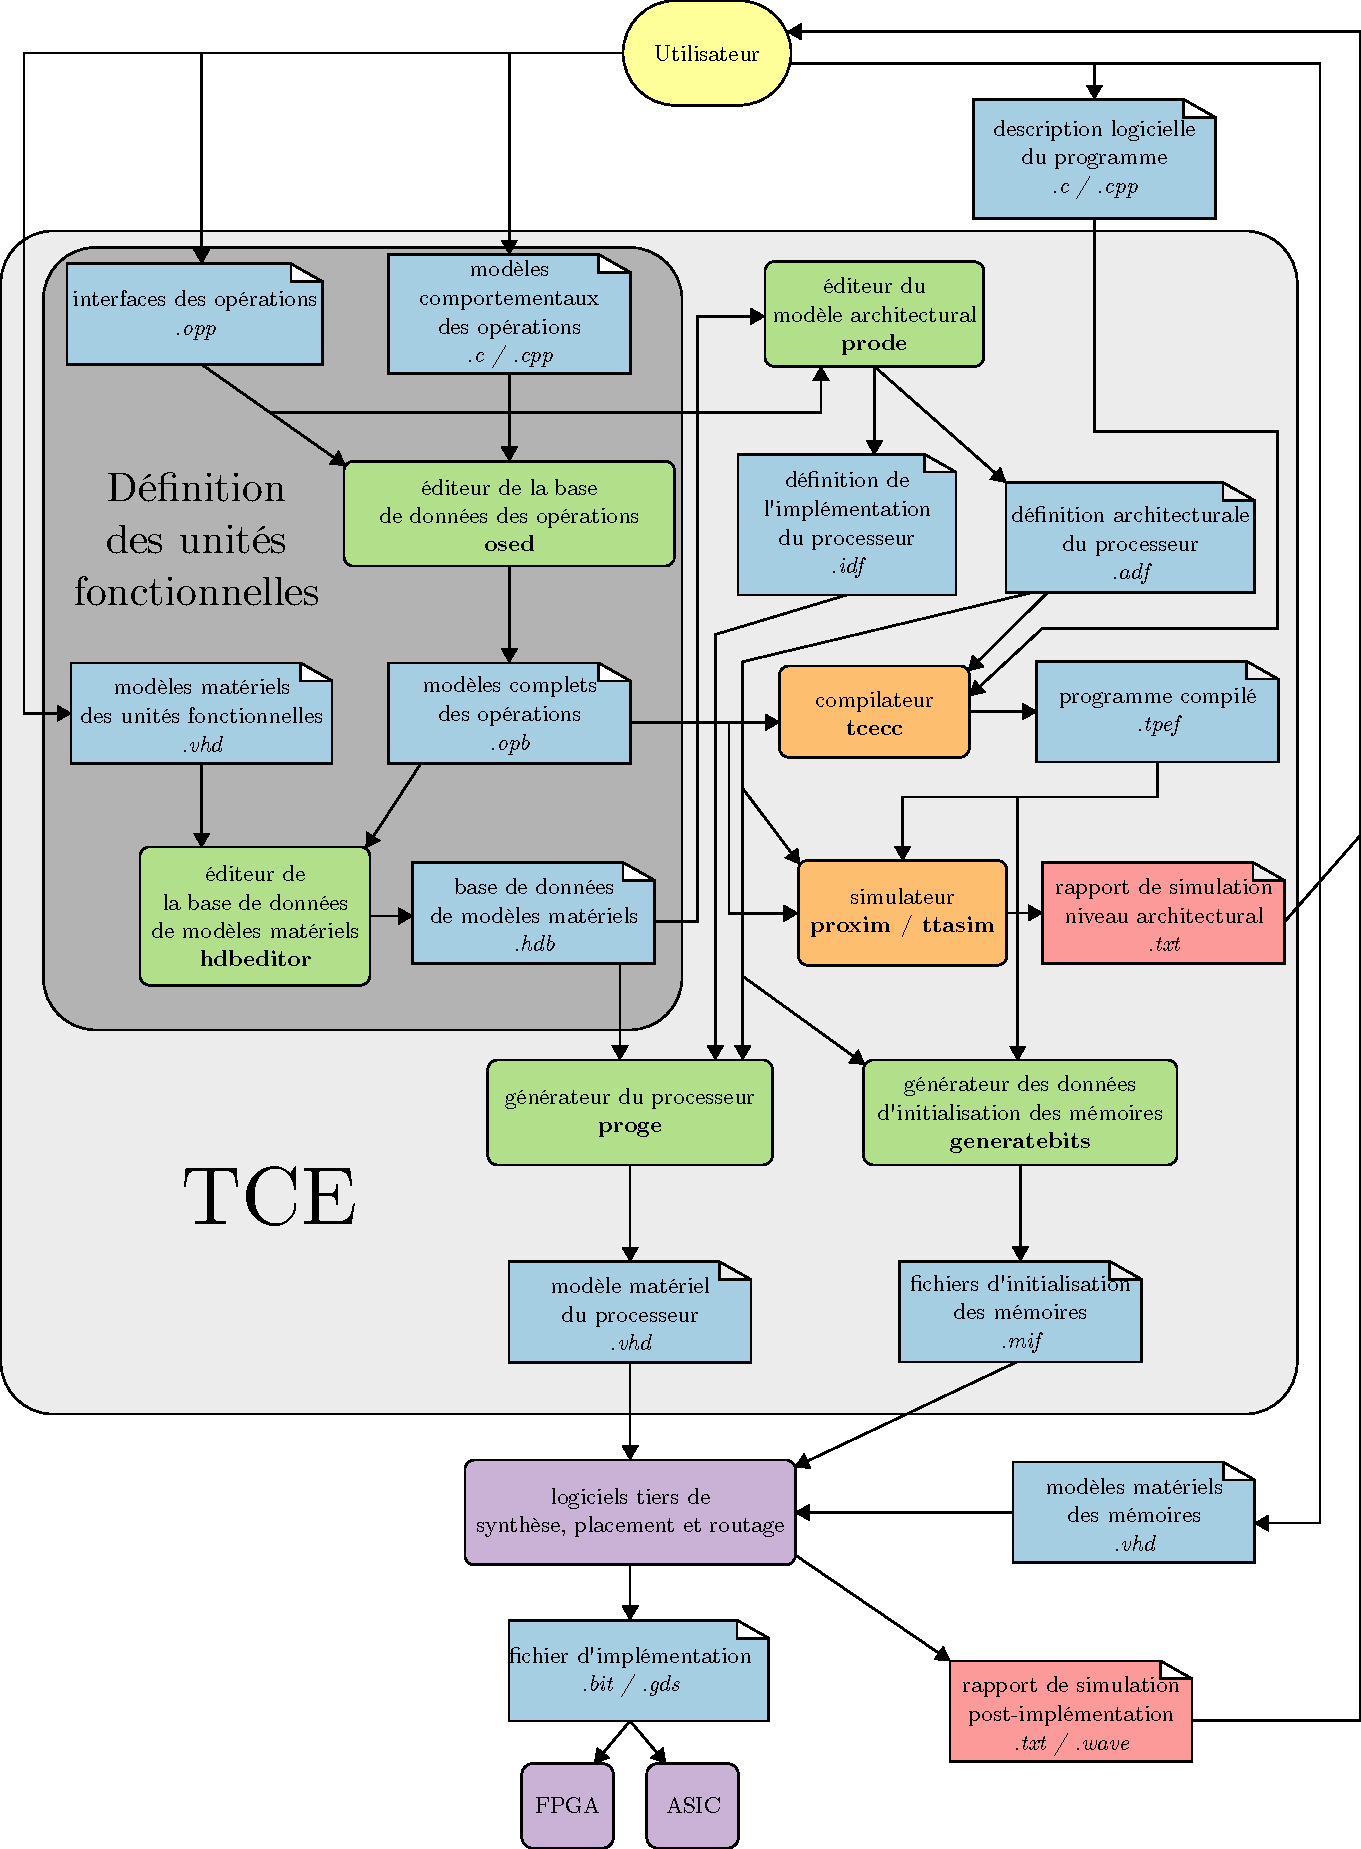
\includegraphics[width=\textwidth]{main/ch4_fig/tce}
\caption{Organisation du flot de conception TCE.}
\label{fig:tce}
\end{figure}
Les modèles matériels des unités fonctionnelles sont décrits en langage VHDL ou Verilog. Un grand nombre de modèles matériels et d'opérations de base sont fournis par la suite logicielle TCE : unités de chargement et de sauvegarde, fichiers de registres, ALU, unités SIMD, interfaces d'entrée et de sortie, entre autres. Pour créer des unités fonctionnelles spécifiques, l'utilisateur doit décrire l'interface des opérations, leurs modèles comportementaux et les modèles matériels des unités fonctionnelles dans un langage de description matériel (VHDL ou Verilog). Ces modèles matériels sont réunis dans une base de données de modèles matériels (\textit{.hdb}). Ils sont éditables et consultables à l'aide de l'outil \textit{hdbeditor}.
Le concepteur, à l'aide de la base de données, peut réutiliser des modèles matériels déjà conçus par lui même ou d'autres contributeurs.

Le deuxième fichier produit par \textbf{prode} est le fichier de définition de l'implémentation \textit{.idf}. Il relie simplement chaque unité fonctionnelle définie dans le fichier \textit{.adf} à son implémentation matérielle contenue dans la base de donnée des modèles matériels.

\subsubsection{Simulation au niveau architectural.}

Le compilateur (\textbf{tcecc}) utilise le fichier de description architecturale \textit{.adf} et les modèles des opérations afin de compiler le programme. Ce programme est écrit dans un langage haut niveau (C, C++, OpenCL). Un effort particulier a été effectué par les développeurs de l'environnement TCE afin de rendre ce compilateur efficace. Il est basé sur le projet LLVM~\cite{lattner_llvm:_2004}. L'environnement TCE bénéficie à ce titre d'optimisations des premiers niveaux de la chaîne de compilation (analyses lexicales, syntaxiques, sémantiques et génération du code intermédiaire). Les dernières étapes d'optimisations spécifiques aux TTAs (dérivation des files de registre, utilisation d'unités fonctionnelles et opérations SIMD) ont été réalisées par les développeurs de l'outil TCE.

Le programme compilé peut ensuite être simulé, soit à l'aide d'un outil en ligne de commandes (\textbf{ttasim}), soit par une interface graphique (\textbf{proxim}). Cette simulation permet d'obtenir le nombre de cycles nécessaires à l'exécution de l'intégralité ou d'une partie du programme, et ainsi d'avoir un premier retour sur l'adéquation entre l'architecture conçue et l'algorithme à exécuter. D'autres fonctions sont disponibles dans ce simulateur. Un profilage permet notamment à l'utilisateur de connaître le nombre de cycles d'exécutions pris par chaque fonction et ainsi de connaître les portions du programme à accélérer en priorité. Le simulateur donne également des métriques importantes, comme l'engorgement des bus, l'engorgement des sockets ou le taux d'utilisation de chaque opération dans les unités fonctionnelles. Cet ensemble de métriques permet au concepteur d'analyser très finement le fonctionnement du processeur conçu et le déroulement du programme.

\subsubsection{Génération du processeur.}

La dernière étape est la génération du modèle matériel complet du processeur. L'outil de génération du processeur (\textbf{proge}) utilise la base de données des modèles matériels des unités fonctionnelles (fichier \textit{.hdb}) ainsi que les fichiers de description de l'architecture et de l'implémentation du processeur (fichiers \textit{.adf} et \textit{.idf}) afin de concevoir l'architecture complète associée au processeur. Elle intègre donc les différents modèles des unités fonctionnelles, le réseau d'interconnexion, mais également l'unité de contrôle, comme illustré dans la Figure~\ref{fig:tta_example}. L'unité de contrôle a pour fonction la lecture du programme, stocké dans la mémoire d'instructions.

L'outil \textbf{generatebits} permet quant à lui de générer les contenus d'initialisation des mémoires de données et d'instructions. Les modèles matériels de ces mémoires doivent être fournis par l'utilisateur. En effet, ceux-ci sont en général dépendants de la cible d'implémentation.

L'architecture du processeur, décrite dans un langage de description matérielle (VHDL ou Verilog) et les modèles des mémoires peuvent ensuite être fournis à un logiciel tiers, pour effectuer la synthèse et l'implémentation sur FPGA ou sur ASIC. Les rapports de synthèse ou d'implémentation fournissent alors des métriques concernant la fréquence de fonctionnement, la surface utilisée et la consommation de puissance. Ces métriques peuvent être utilisées par le concepteur afin d'améliorer l'architecture du processeur. Des itérations du flot de conception permettent d'améliorer le processeur jusqu'à l'obtention de performances satisfaisantes.



\section{Transport Triggered Polar Decoders}
\label{sec:tta_design}

Deux architectures de processeurs spécialisées dans le décodage de codes polaires ont été conçues. Elles sont successivement détaillées dans cette section. La première est spécialisée pour le décodage SC. Elle est nommée \TTSC. Les algorithmes SC et SCAN sont tous deux supportés par la seconde architecture. Celle-ci est nommée \TTSCAN.

\subsection{Architecture du décodeur \TTSC.}

\begin{figure*}[t]
	\centering
	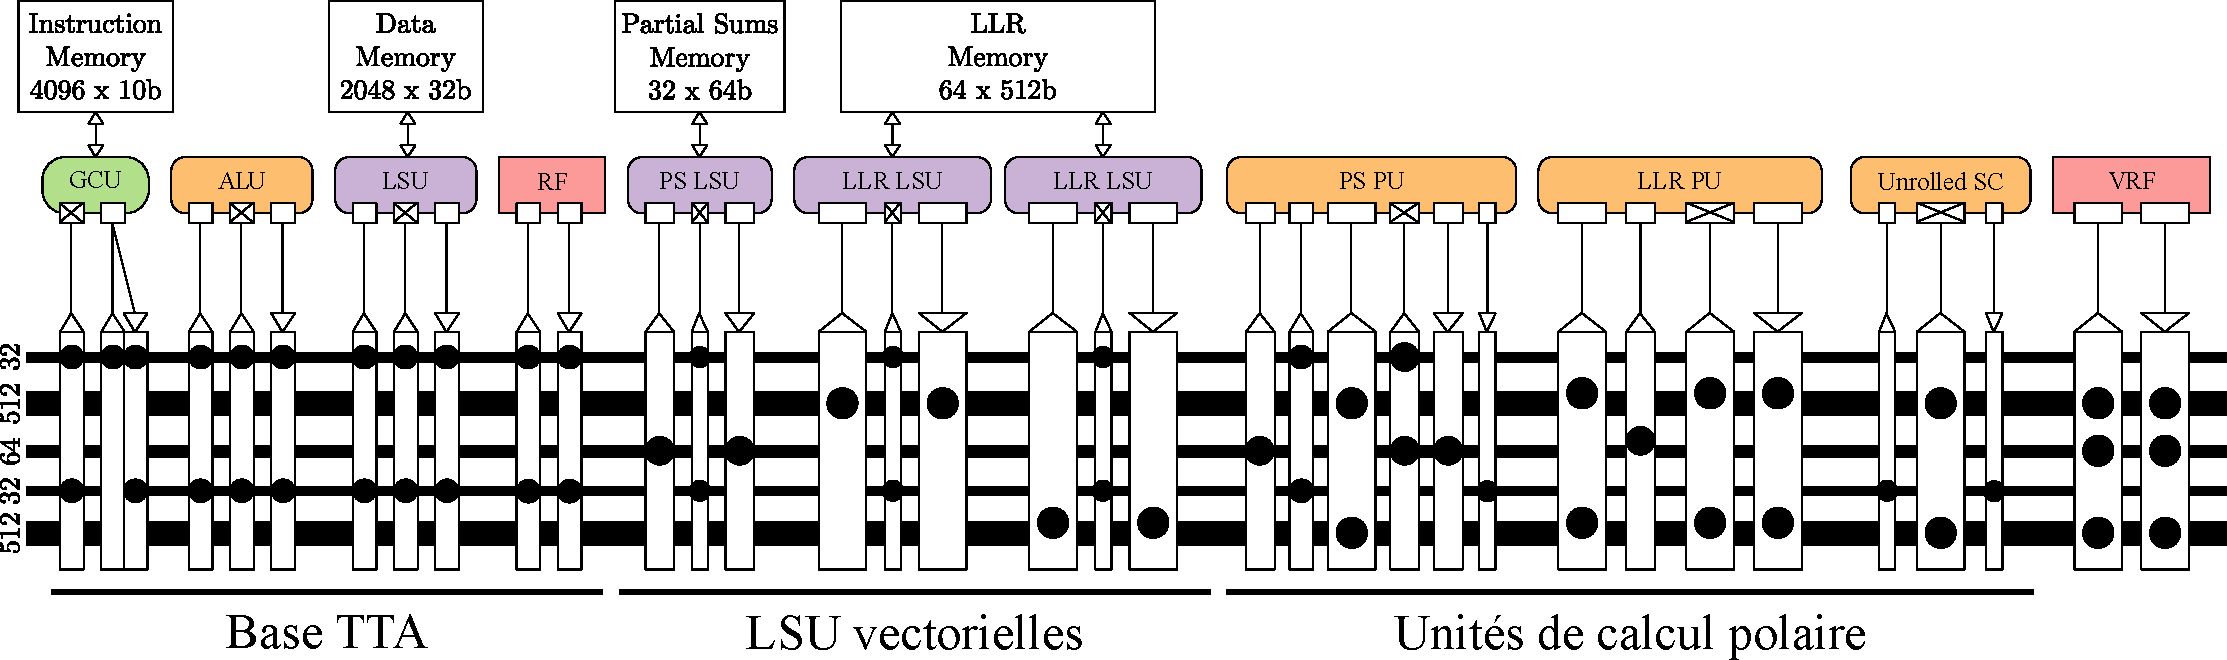
\includegraphics[width=\textwidth]{main/ch4_fig/archi_sc}
	\caption{Architecture \TTSC.}
	\label{fig:prode}
\end{figure*}

Comme illustré dans la Figure~\ref{fig:prode}, l'architecture \TTSC~se compose de trois parties principales. La \textit{Base TTA} contient les unités fonctionnelles de base permettant de réaliser les fonctions d'un processeur généraliste. Elle est constituée d'une unité de chargement et de sauvegarde (LSU : Loading and Storing Unit), d'une ALU et d'une file de registres (RF : Register File). Elle contient également l'unité de contrôle global (GCU : Global Control Unit) qui est destinée à la lecture et au décodage des instructions. La seconde partie est constituée des LSU vectorielles. Elles réalisent les chargements et les sauvegardes des données depuis et vers les mémoires contenant les LLR et les sommes partielles.
La troisième partie contient les unités de calcul (PU : Processing Unit), qui sont en charge de réaliser les fonctions élémentaires polaires.

Les algorithmes de décodages de codes polaires requièrent un grand nombre d'accès à la mémoire. Les architectures matérielles dédiées de la littérature utilisent en majorité deux mémoires séparées pour accéder aux LLR et deux autres pour les sommes partielles. Pour l'opération $f$, il est par exemple nécessaire d'effectuer deux lectures en mémoire ainsi qu'une écriture. Lorsque le parallélisme ($P=64)$ est pris en compte, le total des accès est de 128 lectures pour 64 écritures. Les mêmes lectures et écritures sont nécessaires pour la fonction $g$, auxquelles il faut ajouter la lecture de 64 sommes partielles. Dans l'architecture \TTSC, nous avons choisi d'utiliser une mémoire double port pour stocker les LLR. Cela permet d'augmenter la bande passante, tout en conservant un seul espace de mémoire pour l'ensemble des LLR. A chaque port est associé une LSU. Une LSU permet de lire ou d'écrire 64 données en mémoire par déclenchement.

Les trois unités de calcul sont l'unité de calcul de sommes partielles (PS PU), l'unité de calcul des LLR (LLR PU) et l'unité \og SC déroulé \fg. La PS PU réalise les calculs des fonctions \texttt{R0}, \texttt{R1} et \texttt{h}. La LLR PU réalise les calculs des fonctions $f$ et $g$. L'unité \og SC déroulé \fg permet le décodage multi-cycles de sous-arbres. Elle sera détaillée par la suite. 

Le nombre d'unités fonctionnelles choisies par le concepteur dans une architecture TTA fait l'objet d'un compromis.
Tout d'abord, une unité fonctionnelle ne peut activer qu'une opération à la fois.
Augmenter le nombre de FUs est donc nécessaire pour bénéficier du parallélisme d'instructions.
Cela permet également d'augmenter la modularité de l'architecture du point de vue du concepteur.
\`A fonctionnalité égale, utiliser un grand nombre de FUs permet de spécialiser chaque FU pour un sous-ensemble d'instructions. Cela simplifie leurs structures. Les modèles matériels sont donc plus simples à décrire, à modifier et à faire évoluer. Il est également plus probable de pouvoir réutiliser une FU simple dans de futures architectures.

En revanche, le nombre de ports augmente avec le nombre de FUs, ainsi que le nombre de connexions nécessaires sur le réseau d'interconnexion.
Au niveau de l'implémentation, la densité du réseau d'interconnexion devient rapidement un problème. 
La congestion peut provoquer une augmentation du chemin critique et donc une diminution de la fréquence d'exécution. 
Au cours du développement de l'architecture \TTSC, il a été nécessaire de fusionner des FUs afin de réduire la congestion et d'augmenter la fréquence d'horloge. Ce fut obtenu au prix d'une réduction de la modularité et d'une augmentation de la complexité des FUs. La PS PU est issue par exemple de la fusion de trois FUs de versions antérieures de l'architecture.

Le réseau d'interconnexion développé possède deux bus de 512 bits pour le transport des LLR, un bus de 64 bits pour le transport des sommes partielles et deux bus de 32 bits pour le transport des données génériques et des adresses.
Dans la sous-section suivante, certaines des FUs sont détaillées.

\subsection{Unités fonctionnelles du décodeur \texttt{TT-SC}.}
Nous détaillons ici la fonction et l'implémentation matérielle de certaines des FUs. Certaines (GCU, ALU, LSU, RF) sont liées au fonctionnement du base du TTA et à ce titre ne sont pas pertinentes dans le contexte de nos travaux. D'autres (LLR PU et PS PU) sont très similaires aux instructions spécialisées de l'architecture de processeur XTensa décrites dans la sous-section~\ref{subsec:multi_reg} du chapitre~\ref{chap:tensilica}.

Les unités fonctionnelles originales spécifiques à l'architecture de processeur TTA sont les unités de chargement et de sauvegarde vectorielles d'une part, et l'unité \og SC déroulé \fg d'autre part.

\subsubsection{Unités de chargement et de sauvegarde.}



Les unités de chargement et de calcul vectoriels permettent d'accéder aux mémoires contenant les LLR et les sommes partielles. Dans l'architecture proposée, la taille de code maximum supportée est $N_{max}=1024$. Il s'agit de la taille maximale définie dans le standard 5G~\cite{3gpp_ts_2017}. Cette valeur peut être facilement ajustée en augmentant la profondeur des mémoires. Dans l'algorithme SC, $N_{max}$ bits sont nécessaires pour stocker les sommes partielles. Puisqu'il est nécessaire d'accéder à $P=64$ sommes partielles en parallèle, une mémoire de 16 x 64-bits est suffisante. Cependant une taille supérieure de mémoire a dû être sélectionnée : 32x64-bits. En effet, une section d'adresse est automatiquement réservée par TCE. Pour des raisons similaires, les LLR sont stockés dans une mémoire de 64x512-bits.

Comme précisé auparavant, l'accès à la mémoire est un enjeu capital dans les architectures de décodage de codes polaires. Les modèles architecturaux et matériels de LSU proposés par défaut dans les bases de données de TCE ont une latence de 3 cycles d'horloge, ce qui ralentit très fortement l’exécution du décodage. C'est pourquoi, cette latence a été réduite à un cycle d'horloge par la suppression de registres. Cette suppression n'a pas affecté la fréquence maximale de fonctionnement.
\begin{figure*}[htp]
	\centering
	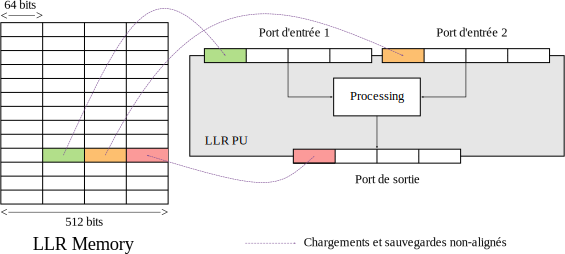
\includegraphics[width=\textwidth]{main/ch4_fig/unaligned}
	\caption{Illustration des chargements et sauvegardes non-alignés.}
	\label{fig:unaligned}
\end{figure*}

La seconde amélioration apportée à ces LSU est l'ajout d'unités matérielles et d'opérations d'alignement. En effet, pour effectuer parallèlement le traitement de certaines portions de l'arbre de décodage pour lequel le parallélisme est inférieur à $P$, il est nécessaire de lire et d'écrire des données non-alignées. Les données non-alignées sont des données dont l'adresse n'est pas un multiple de 512, dans le cas des LLR, ou de 64, dans le cas des sommes partielles. De plus, les mots en mémoire sont des mots de 512 bits. Dans les portions de l'arbre à parallélisme inférieur à $P$, il est nécessaire d'écrire des sous-mots de taille inférieure à 512 bits (jusqu'à 64 bits). Il est donc nécessaire que les mémoires gèrent ces écritures de sous-mots. Par ailleurs, les LSUs doivent être capables d'effectuer le contrôle de ces mémoires. Le processus de chargement et de sauvegarde de données non-alignées est illustré dans la Figure~\ref{fig:unaligned}. Dans celle-ci, des sous-mots de 64 bits sont extraits de la mémoire et positionnés en première position des ports d'entrées de la LLR PU. Le traitement est alors réalisé sur les deux ports d'entrée, le résultat est stocké dans le premier sous-mot du port de sortie. Celui-ci est stocké dans la mémoire, dans le quatrième sous-mot de la ligne de mémoire considérée.

\subsubsection{Décodage d'un sous-arbre déroulé multi-cycles.}

Comme cela a été mis en évidence dans~\cite{gal_scalable_2016}, le parallélisme disponible dans le décodage SC varie en fonction de la zone de l'arbre de décodage. Les zones proches du haut de l'arbre disposent d'un très fort parallélisme alors que le bas de l'arbre souffre d'un défaut de parallélisme. Considérons les sous-arbres du bas dont le \noeud racine contient 8 LLR. Ce type de sous-arbre étant de taille réduite, il est possible de le dérouler complètement. Il est montré que ce déroulage permet de réduire le nombre de cycles nécessaires au traitement de ce type de sous-arbre. En effet, la durée de cette séquence de décodage avec une architecture semi-parallèle classique serait de 14 cycles. En déroulant l'arbre de décodage et en découpant le chemin combinatoire à l'aide de registres, la latence résultante n'est plus que de six cycles. Cette technique s'inspire de la technique~\cite{giard_unrolled_2015}. Dans notre cas, le décodeur déroulé n'est pas pipeliné. Le but des registres est simplement de découper le chemin critique afin de garantir une fréquence de fonctionnement suffisante. Comme il n'y a pas de parallélisme temporel, les registres ne sont pas nécessaires. Le chemin de données qui parcourt le sous-arbre de décodage de bout en bout est un chemin multi-cycles.

\begin{figure*}[htp]
	\centering
	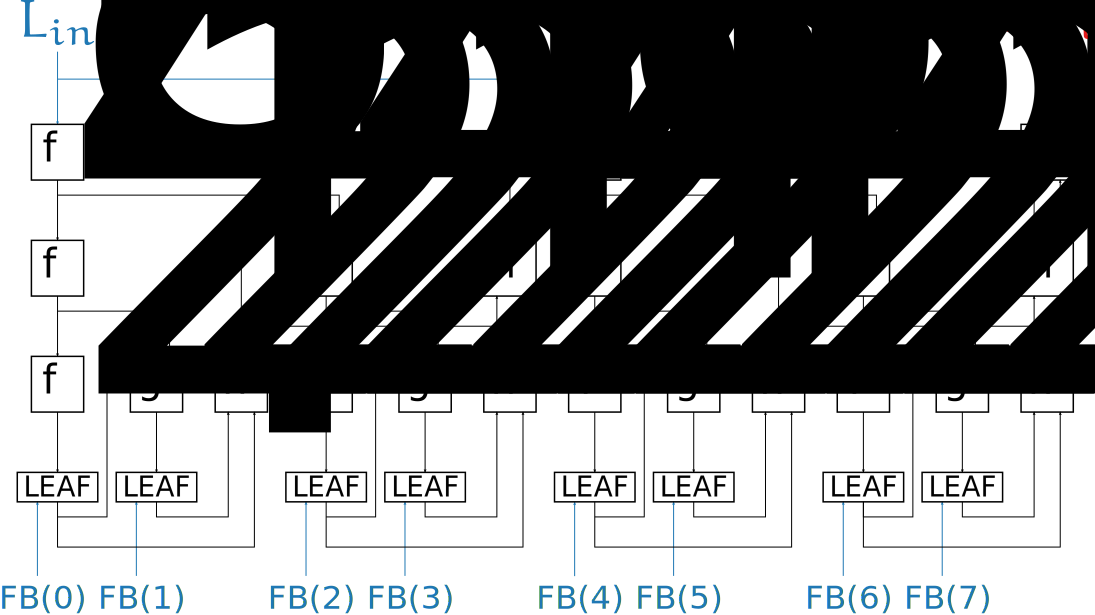
\includegraphics[width=\textwidth]{main/ch4_fig/unrolled_multicycle}
	\caption{Unité matérielle de décodage d'un sous-arbre avec un traitement multi-cycles.}
	\label{fig:unrolled_multicycles}
\end{figure*}

En effet, il est possible de définir des chemins de données multi-cycles dans les processeurs conçus à l'aide de TCE. Par défaut, la latence d'une opération effectuée dans une FU est de un cycle d'horloge : à un front d'horloge, si une donnée est présentée au port de déclenchement, alors les résultats de l'opération sont disponibles aux ports de sortie au front d'horloge suivant. Dans l'outil \textbf{prode}, qui permet de définir l'architecture, il est toutefois possible d'assigner une latence supérieure à une ou plusieurs opérations d'une FU. Si une latence supérieure est spécifiée, alors les données de sortie ne seront disponibles qu'après le nombre spécifié de cycles d'horloge. Le compilateur a connaissance de cette latence spécifiée dans le fichier \textit{.adf}. Il est ainsi en charge de régler les problèmes de disponibilité des données. Du côté du logiciel de synthèse tiers, il faut spécifier que les chemins de données de l'opération en question sont multi-cycles. Leur contrainte de temps est allongée de plusieurs cycles d'horloge. Ainsi, aucun registre n'est assigné et la complexité matérielle de l'unité n'est pas impactée. Cette technique permet de réduire le nombre de cycles nécessaires au décodage du sous-arbre par rapport à la version contenant les registres.

L'unité fonctionnelle \og SC déroulé \fg correspond donc à un sous-arbre de décodage SC déroulé et multi-cycles. Cette unité est détaillée dans la Figure~\ref{fig:unrolled_multicycles}. Il est important de noter que les bits gelés sont donnés en entrée du sous-arbre. Cela permet d'être générique vis-à-vis du rendement et de la construction du code polaire.

\subsection{Description logicielle ciblant l'architecture \TTSC~conçue.}

La notion de déroulage de code source a été présentée dans la sous-section~\ref{subsec:unroll}. Dérouler le code source permet de réduire le nombre de calculs d'adresse et le nombre d'indirections. Durant la conception de l'architecture \TTSC, les indirections sont devenues problématiques. Souvent, celles-ci causaient une sous-utilisation des différents bus. Le traitement d'une indirection nécessite en effet plusieurs cycles d'horloges. De manière récurrente, les bus de transports et les unités fonctionnelles étaient inactives durant ces cycles d'horloge. Le déroulage du code a permis de lever ce verrou. Cependant, le déroulage du code n'est pas sans conséquence. Lorsque l'arbre de décodage est élagué, un code source doit être compilé pour chaque construction du code.

Pour cela, la bibliothèque proposée dans~\cite{cassagne_efficient_2015} a été utilisée. L'intérêt de cette bibliothèque est de faciliter la génération de codes sources déroulés (en langage C++). Les cibles architecturales visées sont les processeurs x86 et ARM. Cette bibliothèque a donc été étendue afin de permettre la génération d'un code source exploitant les instructions TTA. Ainsi, il est possible de générer le code source déroulé et élagué de n'importe quelle construction de code polaire, quels que soient la taille et le rendement. Par ailleurs, de manière équivalente aux décodeurs logiciels à liste proposés dans le chapitre~\ref{chap:soft_scl}, l'élagage de l'arbre est ajustable, en fonction du type de \noeuds utilisés ou de la taille des \noeuds activés.


\begin{figure}[t]
\centering
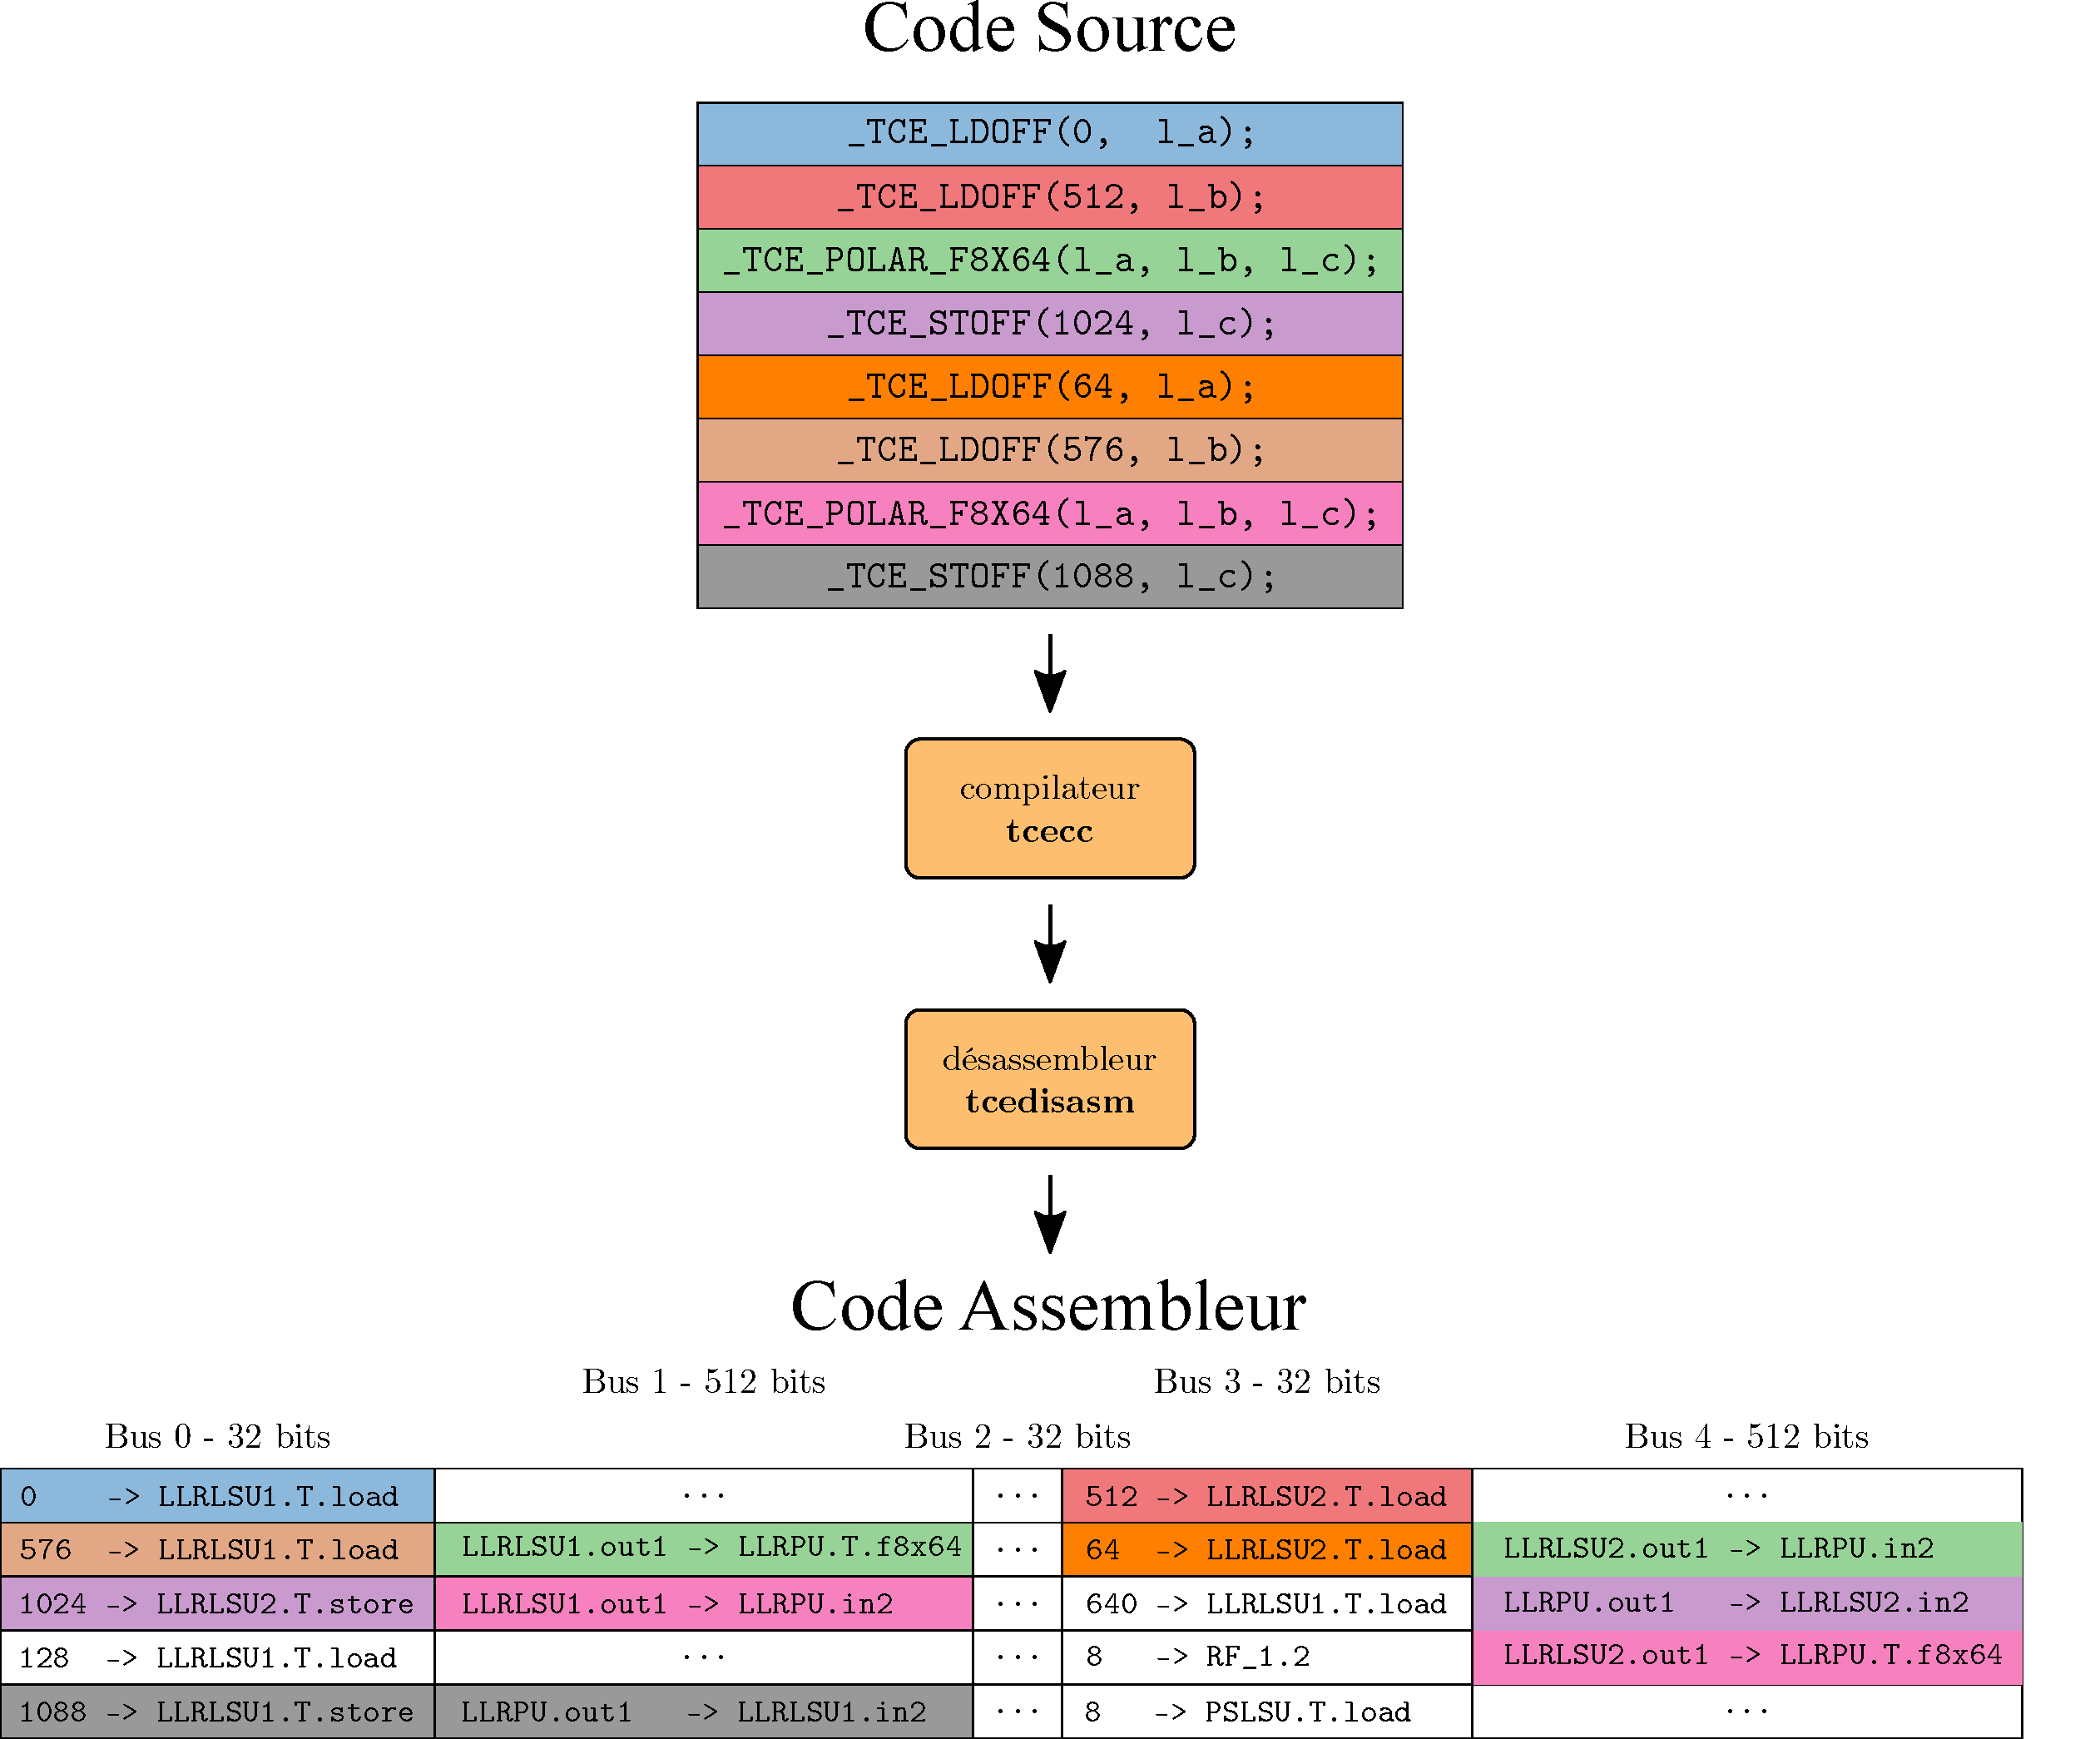
\includegraphics[width=\textwidth]{main/ch4_fig/ilp_1}
\caption{Exemple d'un code source et du code assembleur résultant.}
\label{fig:ilp_1}
\end{figure}


La Figure~\ref{fig:ilp_1} contient une illustration du code source. Il s'agit du traitement des premiers \noeuds de l'arbre. Des données sont chargées depuis la mémoire (\texttt{\_TCE\_LDOFF}), la fonction $f$ est appliquée (\texttt{\_TCE\_POLAR\_F8X64}), puis le résultat est stocké dans la mémoire (\texttt{\_TCE\_STOFF}). Le désassembleur de TCE permet de visualiser le code assembleur correspondant au programme généré par le compilateur. Il apparaît clairement que grâce à la génération du code source déroulé, le compilateur exploite efficacement les possibilités de parallélisme d'instructions offertes par les processeurs TTA. Dans cet exemple, la moyenne du nombre d'unités fonctionnelles déclenchées par cycle d'horloge est de 2. Les bus 0 et 3 sont utilisés à 100\%, les bus 1 et 4 sont utilisés à 60\% et le bus 2 n'est pas utilisé. En effet, à ce stade de l'algorithme de décodage, aucune opération n'est appliquée sur les sommes partielles. Durant le décodage d'un mot de code (1024,512), les bus sont occupés à 45\% et le nombre moyen d'unités fonctionnelles actives par cycle d'horloge est de $1.4$. En analysant finement le code source, il y a principalement deux cas de figure où les bus et les unités fonctionnelles sont peu occupés. Le premier correspond aux sections où les unités \og SC déroulé \fg multi-cycles sont activées. 
\begin{figure}[htp]
\centering
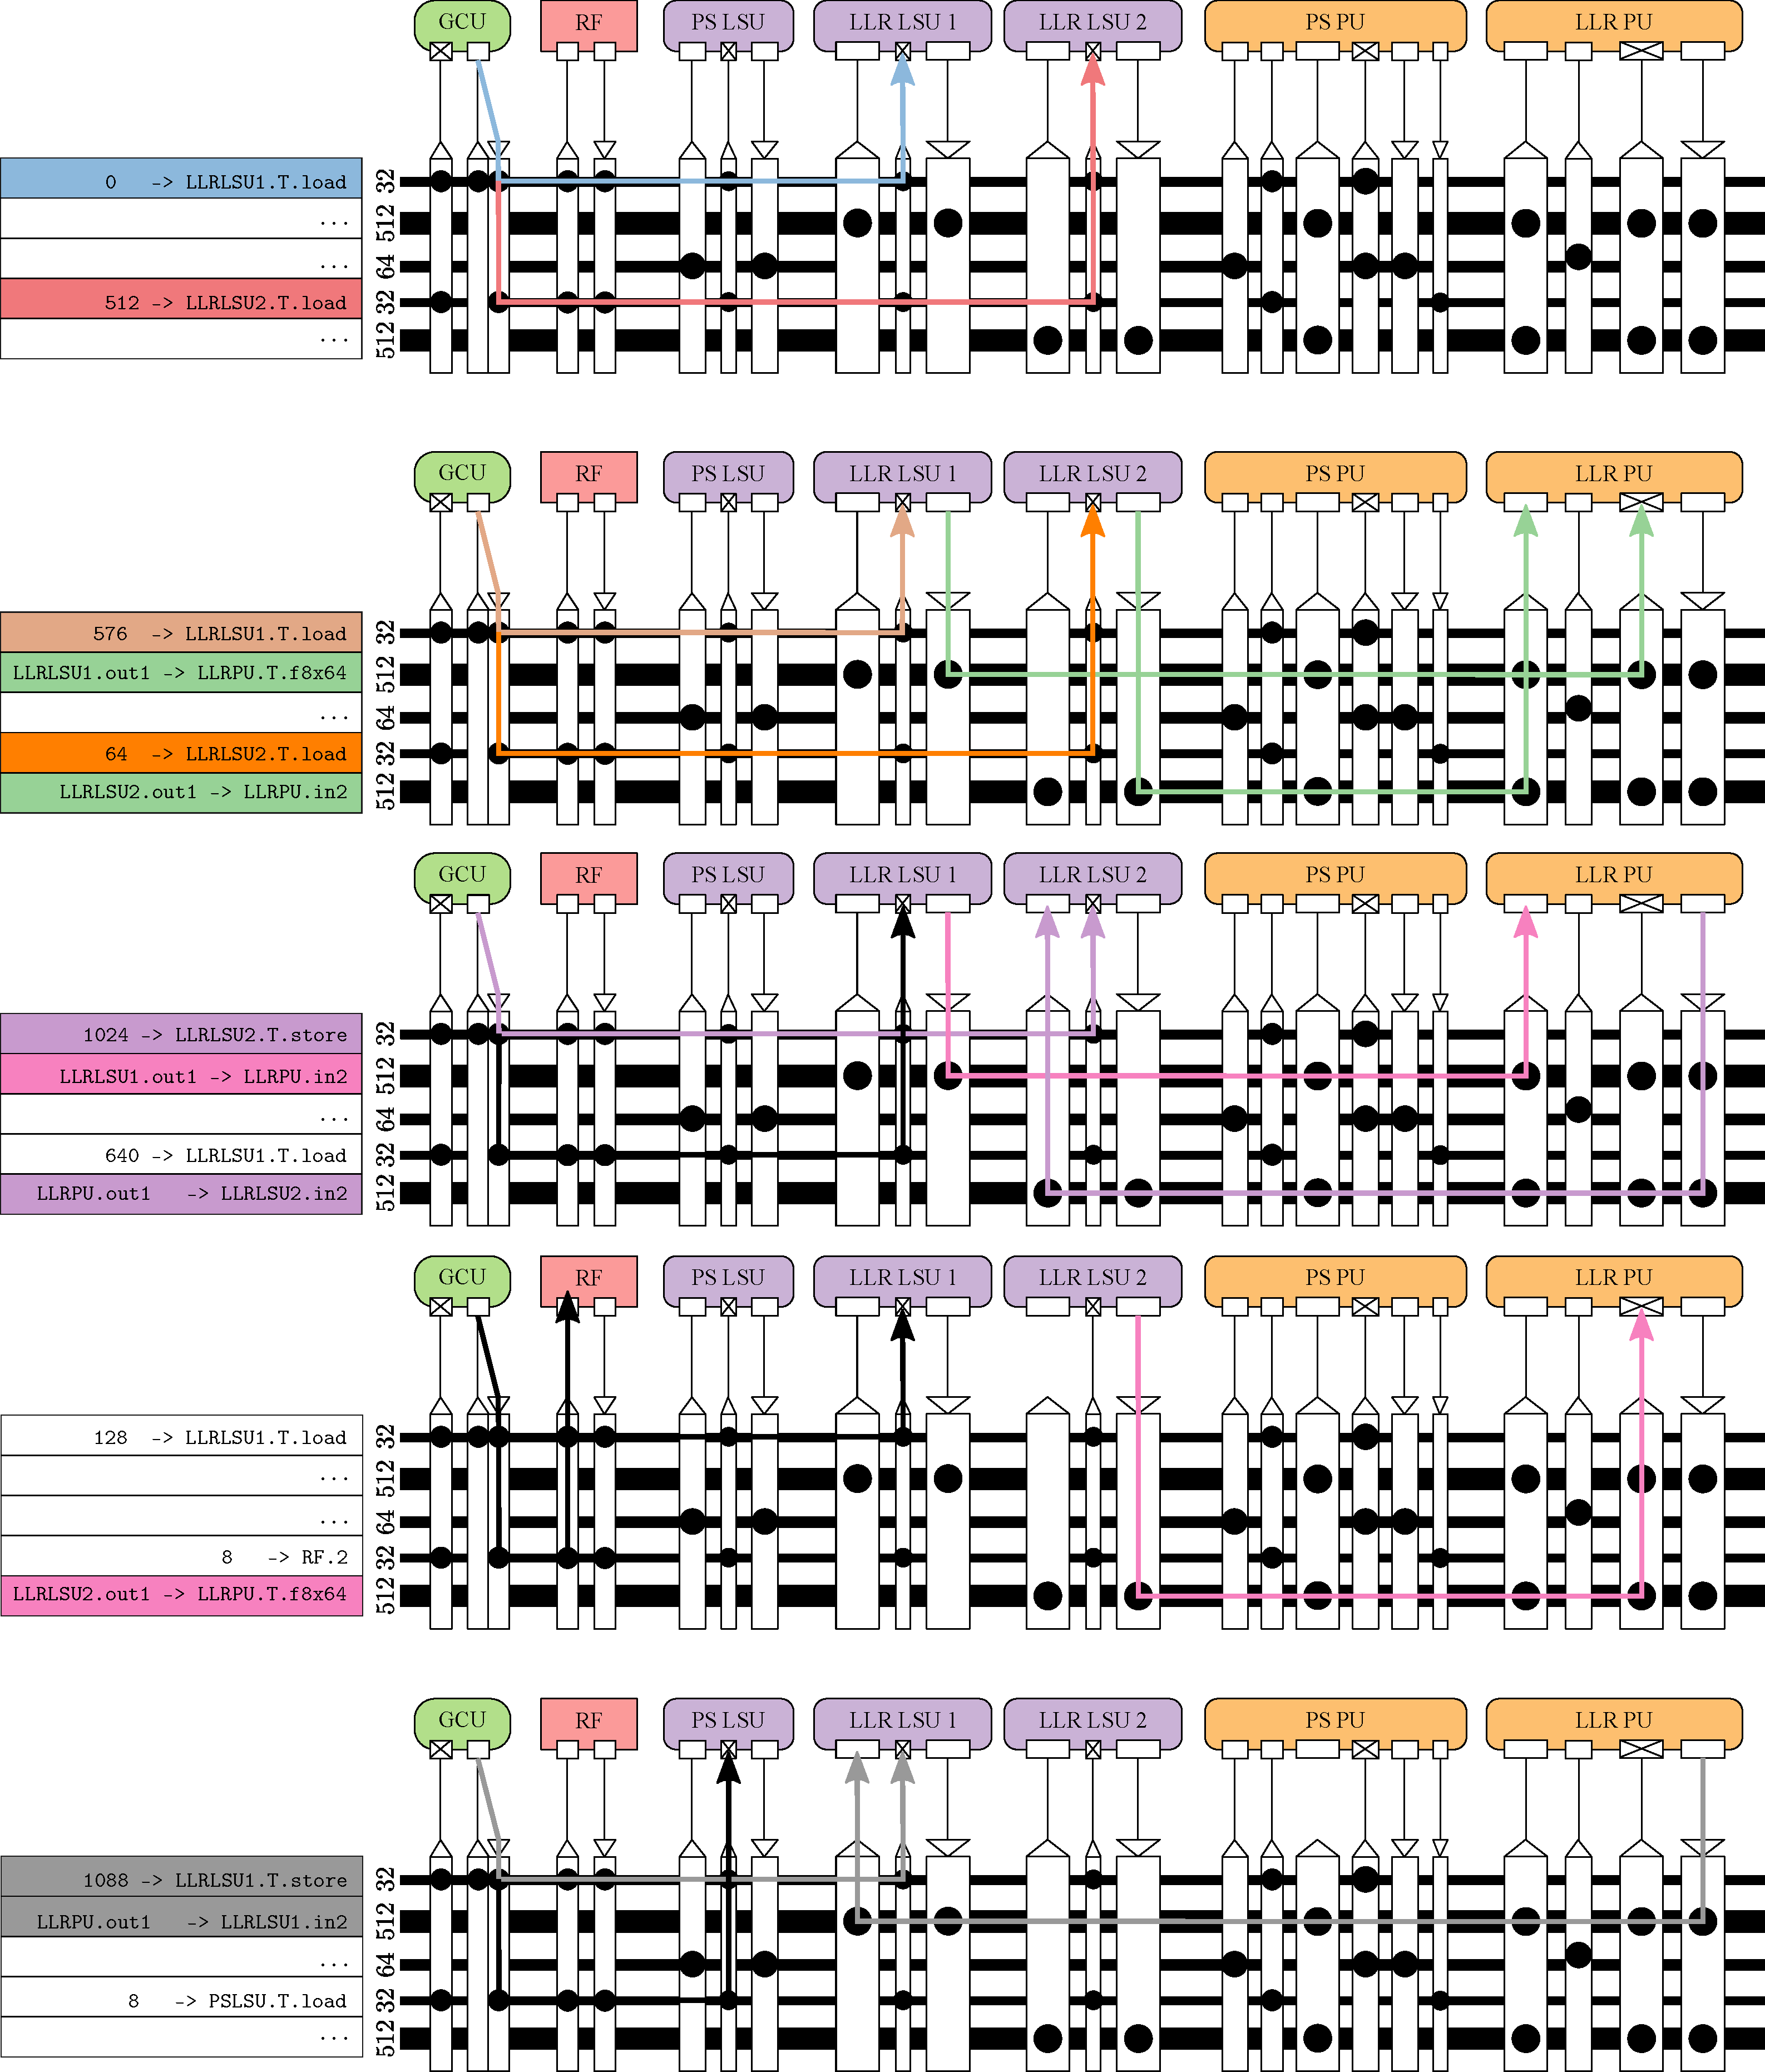
\includegraphics[width=\textwidth]{main/ch4_fig/ilp_2}
\caption{Illustration du parallélisme d'instructions sur le processeur \TTSC.}
\label{fig:ilp_2}
\end{figure}
Le second correspond à la propagation des sommes partielles dans l'arbre. En effet, un seul bus est disponible pour les sommes partielles. De plus, une seule LSU est allouée au stockage et au chargement des sommes partielles. Des améliorations de l'architecture seraient donc possibles afin d'augmenter le taux d'utilisation des bus et des unités fonctionnelles. Cela permettrait de réduire le nombre de cycle d'horloges nécessaires au décodage d'un mot de code.

Une illustration de l'exécution d'un programme par le processeur \TTSC~est donnée dans la Figure~\ref{fig:ilp_2}. Les transports de données sont explicités au cours des cinq cycles d'instructions.



\subsection{Implémentation de l'algorithme SCAN}

\begin{figure}[htp]
	\centering
	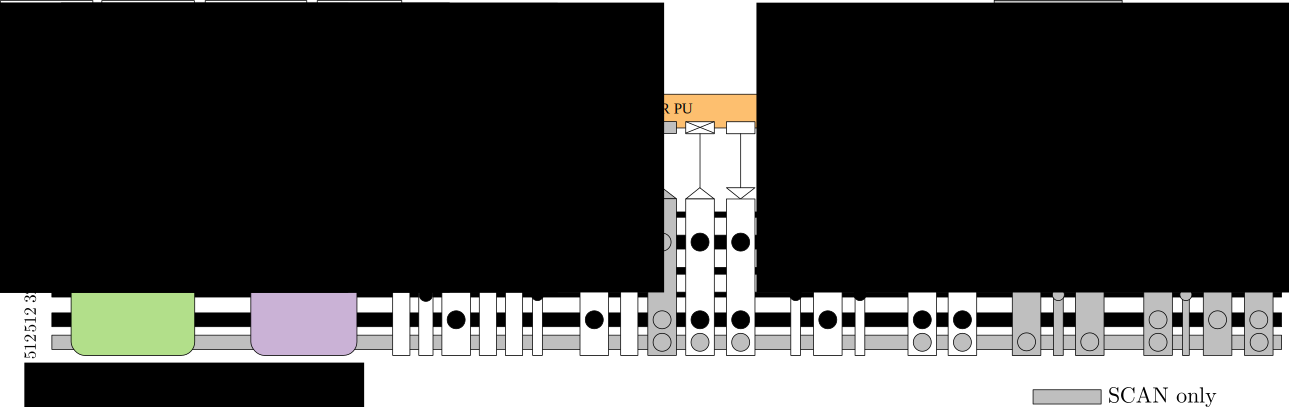
\includegraphics[width=\textwidth]{main/ch4_fig/archi_scan}
	\caption{Architecture \TTSCAN.}
	\label{fig:tt_scan}
\end{figure}
\begin{figure}[htp]
\centering
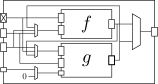
\includegraphics[scale=1.5]{main/ch4_fig/scan_unit}
\caption{Organisation de l'unité \og LLR PU \fg réalisant les fonctions élémentaires SC et SCAN.}
\label{fig:scan_unit}
\end{figure}

Afin d'illustrer la modularité et l'évolutivité des processeurs TTA conçus à l'aide de TCE, nous avons développé une seconde architecture nommée \TTSCAN. Elle permet le support de l'algorithme SCAN en plus de l'algorithme SC. Cette dernière est décrite dans la Figure~\ref{fig:tt_scan}.
Comme détaillé dans la sous-section~\ref{subsec:soft_algo}, les sommes partielles sont remplacées par des LLR dans l'algorithme SCAN. Ces LLR sont notés BLLR (Backward LLR). La première unité fonctionnelle ajoutée à l'architecture \TTSC~pour obtenir l'architecture \TTSCAN~est l'unité de chargement et de sauvegarde des BLLR. Une mémoire de stockage pour les BLLR a également été ajoutée. La seconde unité fonctionnelle ajoutée est une unité \og SCAN déroulé \fg. Cette unité permet d'accélérer le traitement des niveaux inférieurs de l'arbre de décodage, de manière analogue à l'unité \og SC déroulé \fg pour l'algorithme SC.

De plus, l'unité de calcul des fonctions polaires LLR PU a été adaptée. Les fonctions élémentaires nécessaires au décodage de l'algorithme SCAN sont : 
\begin{eqnarray}
  \begin{array}{l c l}
    f_{scan}(L_a,L_b,L_c) & = & f(L_a, L_b  + L_c) \\
    g_{scan}(L_a,L_b,L_c) & = & f(L_a, L_c) + L_b
  \end{array}
  \label{eq:bp}
\end{eqnarray}


Il est possible d'adapter l'unité fonctionnelle LLR PU utilisée dans l'architecture \TTSC~pour qu'elle puisse supporter ces nouvelles fonctions polaires. L'organisation de l'unité matérielle adaptée est illustrée dans la Figure~\ref{fig:scan_unit}. Il est à noter que des multiplexeurs supplémentaires sont nécessaires pour contrôler le paramétrage. Le nombre de cellules logiques nécessaires pour réaliser l'unité fonctionnelle \og SC+SCAN \fg est de 133 sur circuit FPGA. Seules 83 cellules logiques sont nécessaires pour l'unité fonctionnelle \og SC \fg. Cela implique une augmentation de 60 \%.



\section{Expérimentations et mesures.}
Le but de cette section est de présenter les mesures et les expérimentations réalisées afin d'évaluer les deux architectures conçues : \TTSC~et \TTSCAN. Il est important de souligner que les comparaisons avec les décodeurs de la littérature sont délicates. En effet, beaucoup de paramètres changent, tels que la technologie d'ASIC, la tension d'alimentation, les algorithmes supportés par les différentes architectures, la stratégie d'élagage, le format de représentation des LLR, la construction du code polaire. Ces précautions prises, nous allons montrer que les architectures TTAs proposées offrent un compromis pertinent entre les architectures de processeur à usage général et les architectures matérielles dédiées. Nous allons montrer également que ces architectures permettent une amélioration significative du débit et une réduction de la consommation énergétique par rapport au processeur XTensa détaillée tout au long du chapitre~\ref{chap:tensilica}.

\subsection{Architecture \texttt{TT-SC}.}
\label{sec:tta_res}

L'architecture \TTSC~a été synthétisée avec la bibliothèque de cellules standard ST 28nm FD-SOI, avec les paramètres 0.9V, 125$^{\circ}$C~\cite{st_fdsoi_2015}. Les mémoires sont des blocs de SRAM de la même technologie. Le Tableau~\ref{tab:sw_tta} présente les performances de débit, latence et consommation de l'architecture \TTSC~exécutant l'algorithme SC. Une comparaison est faite avec les performances obtenues sur des processeurs à usage général d'architectures x86 et ARM, ainsi qu'avec celles obtenues sur le processeur XTensa du chapitre~\ref{chap:tensilica}.


\begin{table}
  \centering
  \caption{Comparaison de l'architecture \TTSC~avec des processeurs à usage général et l'ASIP XTensa proposé dans le chapitre~\ref{chap:tensilica}.}
  \label{tab:sw_tta}
%\scriptsize
  \begin{tabular}{ccccc}
    \toprule

    Architecture & $N$ & \begin{tabular}{c}Latence\\{[$\mu$s]}\end{tabular} & \begin{tabular}{c}Débit\\{[Mb/s]}\end{tabular} & \begin{tabular}{c}$E_b$\\{[nJ/bit]}\end{tabular} \\

    \cmidrule(lr){1-1}
    \cmidrule(lr){2-2}
    \cmidrule(lr){3-5}

    \multirow{2}{*}{\bf i7-3.3GHz}              & $1024$   & $2.0$  & $257$ & $41$ \\
    
                                                & $512$    & $1.2$  & $210$ & $49$ \\
    
    \multirow{2}{*}{\bf (GPP)}                  & $256$    & $0.7$  & $179$ & $59$ \\
    
                                                & $128$    & $0.4$  & $143$ & $73$ \\
    
    \midrule    \multirow{2}{*}{\bf A57-1.1GHz} & $1024$   & $10.7$ & $48$  & $17$ \\

                                                & $512$    & $5.3$  & $48$  & $17$ \\

     \multirow{2}{*}{\bf (GPP)}                 & $256$    & $2.8$  & $46$  & $17$ \\

                                                & $128$    & $1.6$  & $41$  & $20$ \\

    \midrule

    \multirow{2}{*}{\bf LX7-835MHz}             & $1024$   & $7.2$  & $71$  & $1.6$ \\

                                                & $512$    & $3.9$  & $66$  & $1.7$ \\

     \multirow{2}{*}{\bf (ASIP)}                & $256$    & $1.9$  & $65$  & $1.7$ \\

                                                & $128$    & $1.0$  & $62$  & $1.8$ \\

    \midrule

    \multirow{2}{*}{\bf TT-SC-800MHz}            & $1024$  & $1.4$   & $352$ & $0.14$   \\ % 1512 cycles

                                                & $512$    & $0.8$  & $313$ & $0.15$   \\ % 803 cycles

     \multirow{2}{*}{\bf (ASIP)}                & $256$    & $0.4$  & $304$ & $0.16$   \\ % 413 cycles

                                                & $128$    & $0.2$  & $284$ & $0.17$   \\ % 224 cycles

    \bottomrule
  \end{tabular}
\end{table}

Pour les deux processeurs à usage général, le code source utilisé est généré à l'aide de la bibliothèque introduite dans~\cite{cassagne_efficient_2015}. Les simulations sont effectuées grâce à la suite logicielle AFF3CT~\cite{cassagne_fast_2017}. Le processeur Intel i7-4712HQ présente un débit élevé mais induit une importante consommation énergétique. Le débit mesuré sur le processeur ARM A57 est moins élevé, mais la consommation énergétique est plus faible que celle obtenue sur le processeur Intel. Comme nous l'avons vu dans le chapitre précédent, le débit obtenu sur le processeur spécialisé XTensa est comparable à celui obtenu sur l'architecture ARM, alors que la consommation énergétique est dix fois plus faible. L'architecture \TTSC~permet d'atteindre un débit plus élevé que les trois autres architectures, tout en réduisant d'un ordre de grandeur la consommation énergétique en comparaison du processeur XTensa. Par exemple, avec un code polaire (1024,512), le débit obtenu par le processeur \TTSC~est de 352 Mb/s, ce qui est supérieur de 37 \% au débit obtenu avec le processeur Intel i7-4712HQ, alors que la consommation énergétique est beaucoup plus faible, avec deux ordres de grandeur de différence. Nous en concluons que l'approche développée dans ce chapitre est pertinente et aboutit à des résultats convaincants.

\begin{table}[t]
  %\renewcommand{\arraystretch}{0.5} 
  %\tabcolsep=6pt
  \centering
  \caption{Implémentations sur cible FPGA de décodeurs SC pour un code polaire (1024,512).}
  \label{tab:fpga_tta}
  \begin{tabular}{rccccc}
   \toprule

                            & \TTSC     &~\cite{giard_638_2015} & \multicolumn{2}{c}{\cite{sarkis_fast_2014}}  \\ % & \texttt{TT-SC-COMP} \\
	\cmidrule(lr){2-2}
	\cmidrule(lr){3-3}
	\cmidrule(lr){4-5}
	% \cmidrule(lr){6-6}

    \textbf{Cible}              &  Artix-7  & Stratix IV            & Stratix IV          & Virtex 6               \\ % & Artix-7             \\
    \textbf{Cycles d'horloge}   &  1161     & 222                   & 165                 & 165                    \\ % & 1161                \\
    \textbf{Débit info.} (Mb/s) &  44       & 238                   & 319                 & 217                    \\ % & 44                  \\
    \textbf{Fréquence} (MHz)    &  100      & 103                   & 103                 & 70                     \\ % & 100                 \\
    \textbf{LUTS}               &  14744    & 23020                 & 24821               & 22115                  \\ % & 17352               \\
    \textbf{FFs}                &  7354     & 1024                  & 5823                & 7941                   \\ % & 7354                \\
    \textbf{RAM} (Kb)           &  948      & 43                    & 36                  & 36                     \\ % & 141                 \\
    \textbf{\'Elagage}          &  R0 \& R1 & Complet               & Complet             & Complet                \\ % & R0 \& R1            \\
    \bottomrule   
  \end{tabular}  
\end{table}

Les performances de l'architecture \TTSC~se rapprochent des performances des architectures matérielles dédiées de l'état de l'art. Le Tableau~\ref{tab:fpga_tta} présente les performances de plusieurs implémentations de l'algorithme SC sur des cibles FPGA. Les deux références~\cite{sarkis_fast_2014,giard_638_2015} sont des implémentations de la version élaguée de l'algorithme (FAST SC). L'élagage est complet, c'est-à-dire que tous les \noeuds spécialisés sont utilisés, en particulier les \noeuds \texttt{REP} et \texttt{SPC}, contrairement à l'architecture \TTSC~dans laquelle seuls les \noeuds \texttt{R1} et \texttt{R0} sont considérés. Le nombre de cycles d'horloge nécessaire au décodage d'un mot de code est 5 fois plus faible pour les architectures dédiées que pour l'architecture \TTSC. Trois facteurs principaux expliquent cette différence. Premièrement, comme il vient d'être expliqué, l'élagage est plus complet dans les architectures dédiées. Cet aspect pourrait être corrigé dans des versions améliorées de l'architecture \TTSC. Deuxièmement, dans l'architecture \TTSC, le chemin constitué d'une lecture en mémoire, d'une opération élémentaire polaire et d'une écriture en mémoire prend trois cycles d'horloge. Dans les architectures dédiées, ces trois opérations sont réalisées en un seul cycle d'horloge. Le compilateur utilise le parallélisme d'instructions pour limiter cette différence, mais ceci n'est pas toujours possible durant le déroulement de l'algorithme de décodage. Troisièmement, comme indiqué dans la sous-section~\ref{subsec:hard_sc}, la propagation des sommes partielles se réalise en parallèle des autres opérations dans les architectures matérielles. Dans l'architecture \TTSC, la propagation des sommes partielles représente environ 20\% du temps nécessaire au décodage d'une trame. Cela impacte donc le coût au niveau du nombre de cycles d'horloge.


Le nombre de LUT utilisées par l'architecture \TTSC~est inférieur à celui des architectures dédiées. La principale raison est que l'architecture \TTSC~ne gère qu'un élagage limité contrairement aux architectures matérielles dédiées considérées. Or, la gestion de l'élagage implique des unités de traitement spécifiques coûteuses en ressources calculatoires. Néanmoins, l'architecture \TTSC~est une architecture de processeur programmable complète, avec une ALU généraliste. La présence de cette ALU généraliste et d'une LSU associée permet à l'architecture TTA de pouvoir potentiellement réaliser n'importe quel algorithme décrit en langage de haut niveau. Si ce nombre réduit de LUT est un fait notable, la versatilité de l'architecture \TTSC~a néanmoins un coût. En effet, le nombre de bascules flip-flop utilisées est supérieur. Beaucoup de registres sont nécessaires dans les architectures TTA, dans chaque unité fonctionnelle. De plus, les instructions utilisées par le processeur \TTSC~sont très longues : une instruction est stockée sur 198 bits. L'empreinte mémoire de la mémoire d'instructions est donc considérable. Cet élément apparaît dans le Tableau~\ref{tab:fpga_tta} en ce qui concerne la quantité de mémoire RAM utilisée. Dans l'architecture proposée, la taille de code polaire maximum est $N_{max}=1024$. $N_{max}$ bits sont nécessaires pour le stockage des sommes partielles. Comme il est nécessaire d'accéder à $P=64$ données en parallèle, une mémoire 16x64-bit est suffisante. Cependant, une zone de mémoire étant réservée par le compilateur, la taille de mémoire supérieure a été sélectionnée : 32x64-bit. Pour des raisons similaires, une mémoire 64x512-bit est utilisée pour les LLR. De plus, il s'agit d'une mémoire double port, son empreinte mémoire est donc doublée. La mémoire de données de 32 bits est une mémoire 2048x32-bit. Au total, l'empreinte mémoire, comprenant également les différents registres vectoriels et scalaires, est de 948 kbits.




\begin{table}[t]
	\begin{centering}
  \caption{Implémentations sur cible ASIC de décodeurs SC pour un code polaire (1024,512).}
	\label{tab:asic_tta}
			\begin{tabular}{rcccc}
				\toprule
				\parnoteclear
				& \texttt{TT-SC-COMP}  &~\cite{giard_polarbear:_2017} &~\cite{mishra_successive_2012} &~\cite{mishra_successive_2012}\parnote{{\footnotesize Les facteurs de mise à l'échelle de 180nm vers 28nm de~\cite{mishra_successive_2012} sont issus de~\cite{giard_polarbear:_2017}.}}
				\\
				\cmidrule(lr){2-2}
				\cmidrule(lr){3-3}
				\cmidrule(lr){4-5}
				
				\textbf{Cible}         &  28nm      & 28nm   & 180nm & 28nm  \\
				\textbf{Cycles d'horloge}   &  1161      & 1833      & 1568  & 1568  \\
				\textbf{Débit info.} [Mb/s]    &  352       & 94        & 49    & 436   \\
				\textbf{Fréquence} [MHz]     &  800       & 336       & 150   & 1335  \\
				\textbf{Puissance} [mW]     &  48       & 18        & 67    & 5     \\
				$\mathbf{E_b}$ [nJ/bit] &  0.14      & 0.19     & 1.4  & 0.011 \\
				\textbf{Surface} [mm$^2$]  &  0.16      & 0.44      & 1.71  & 0.04  \\
				\textbf{\'Elagage}       &  R0 \& R1  & First R0  & None  & None  \\
				
				\bottomrule
			\end{tabular}
			\parnotes
	\end{centering}
\end{table}

85 \% de cette empreinte mémoire est due à la mémoire d'instructions. Nous avons donc étudié des moyens de réduire cette empreinte. Les programmes de décodage utilisent un faible nombre d'instructions différentes. Une optimisation consiste alors à tenter de réduire la taille des instructions à 11 bits seulement en ajoutant un décodeur d'instructions qui permet de convertir des instructions de 11 bits en instructions de 198 bits. La complexité de ce convertisseur est faible, il représente moins de 5\% de la surface totale de l'ASIP. Fonctionnellement, l'architecture \TTSC~modifiée devient alors équivalente à celle des architectures dédiées. Cette architecture modifiée a été synthétisée dans la technologie ST précédemment présentée. Les résultats sont présentés dans le Tableau~\ref{tab:asic_tta}. Cette nouvelle version de l'architecture est nommée \texttt{TT-SC-COMP} (pour \og compressé \fg). Ses caractéristiques sont comparées avec des résultats de décodeurs ASIC de la littérature. La comparaison est toutefois difficile compte tenu de la diversité des paramètres d'implémentations. En effet, le décodeur SC proposé dans~\cite{giard_polarbear:_2017} constitue la base d'un décodeur SCL. Sa puissance et sa surface pourraient donc être réduites si seulement l'algorithme SC était supporté. De plus, une stratégie simpliste d'élagage est utilisée. Ceci explique le débit plus faible que celui obtenu avec l'architecture \texttt{TT-SC-COMP}. Le décodeur SC implémenté dans~\cite{mishra_successive_2012} utilise une technologie ASIC différente et aucun élagage n'est utilisé. Aussi, l'objet du Tableau~\ref{tab:asic_tta} est simplement de montrer que l’architecture \texttt{TT-SC-COMP}~présente une complexité matérielle et une consommation énergétique raisonnable lorsqu'elle est comparée à des implémentations similaires. Elle permet d'atteindre plusieurs centaines de Mb/s tout en conservant la flexibilité d'un processeur programmable.


\subsection{Architecture \texttt{TT-SCAN}.}

Les résultats de l'expérimentation de l'architecture \TTSCAN~sont présentés dans le Tableau~\ref{tab:scan_tta}. La seule implémentation sur circuit FPGA de la littérature est proposée dans~\cite{berhault_hardware_2015}. L'architecture \TTSCAN~ est très proche de celle-ci en terme de nombre de cycles d'horloge, de fréquence et de débit. Elle est toutefois plus complexe au niveau des ressources matérielles, comme en atteste les nombres de LUT et de portes flip-flop utilisées. Cette complexité est due au fait que l'arbre de décodage est élagué, ainsi qu'au niveau de parallélisme qui vaut $P=16$ dans~\cite{berhault_hardware_2015}, contre $P=64$ dans l'architecture \TTSCAN. Du point de vue de l'empreinte mémoire, la différence entre l'architecture \TTSC~et l'architecture \TTSCAN~est due à l'ajout de la mémoire de stockage des BLLR : 256x512-bit.

Une implémentation ASIC de l'algorithme SCAN est proposée dans~\cite{lin_reduced_2015}. Comme pour l'architecture \TTSCAN, l'arbre de décodage est élagué. Dans cette implémentation, le parallélisme est cette fois $P=64$. Dans ce cas, nous constatons que le rapport du nombre de cycles est d'environ 4, ce qui se rapproche de la différence observée entre l'architecture \TTSC~et les architectures dédiées au décodage de l'algorithme SC.

\begin{table}[t]
  %\renewcommand{\arraystretch}{0.5} 
  %\tabcolsep=6pt
  \centering
  \caption{Implémentations sur cible FPGA de décodeurs SCAN pour un code polaire (1024,512).}
  \label{tab:scan_tta}
  \begin{tabular}{rccc}
   \toprule
     & \TTSCAN  &~\cite{berhault_hardware_2015} &~\cite{lin_reduced_2015} \\
	\cmidrule(lr){2-2}
	\cmidrule(lr){3-3}
	\cmidrule(lr){4-4}

    \textbf{Cible}            &  Artix-7      & Stratix IV & ASIC 90nm \\
    \textbf{Cycles d'horloge} &  10755        & 10304      & 2441      \\
    \textbf{Débit info.} (Mb/s)      &  4.5          & 4.4        & 217       \\
    \textbf{Fréquence} (MHz)       &  93           & 90         & 571       \\
    \textbf{LUTS}             &  20602    & 3517       & -         \\
    \textbf{FFs}              &  8520    & 1024       & -         \\
    \textbf{RAM} (Kb)         &  1079         & 209        & -         \\
    \textbf{\'Elagage}          &  R0 \& R1 & Aucun         & R0 \& R1  \\
    \bottomrule
  \end{tabular}  
\end{table}


% \section{Un flot de conception complet}
% \subsection{Génération des vecteurs de tests}
% \subsection{Cycles de conception}


\section{Synthèse}


Dans ce chapitre, deux architectures de processeurs à haute performance pour le décodage des codes polaires SC et SCAN sont successivement présentées. Pour ce faire, le modèle architectural TTA est décrit ainsi que la suite logicielle TCE qui propose un flot de conception complet. TCE permet la génération du modèle matériel du processeur, ainsi que la compilation de programmes décrits dans des langages de haut niveau (C / C++). Cette suite logicielle est utilisée afin de concevoir les deux architectures. Plusieurs contributions originales se dégagent de ce travail.

\begin{enumerate}[label=(\roman*)]
  \item La première architecture de processeur de type TTA spécialisée dans le décodage de codes polaires est proposée.
  \item Une unité matérielle de décodeur SC déroulé et multi-cycles est introduite pour décoder des parties de l'arbre de décodage.
  \item Son équivalent est défini pour l'algorithme de décodage SCAN.
  \item Une unité de calcul supportant les fonctions élémentaires des deux algorithmes SC et SCAN est proposée. Une grande partie des ressources matérielles nécessaires sont mutualisées. L'unité matérielle supportant les deux algorithmes est 60\% plus complexe que celle gérant seulement l'algorithme SC.
  \item L'ASIP ainsi conçu présente des débits supérieurs à ceux obtenus sur des architectures de processeurs à usage général, et la consommation énergétique est réduite de deux ordres de grandeur. Les performances de débits et de consommation énergétique se rapprochent des architectures dédiées tout en conservant une meilleure programmabilité.
\end{enumerate}

Les travaux présentés dans ce chapitre ont été valorisés à travers une publication à la conférence ISTC 2018~\citemine{leonardon_tta_2018}.

L'algorithme SCL permet d'atteindre de meilleures performances que les algorithmes SC et SCAN. Il sera sans doute utilisé dans le cadre du standard 5G. Aussi, de futurs travaux se concentreront sur la conception d'une architecture TTA supportant l'algorithme SCL. De plus, la suite logicielle TCE facilite la conception d'architectures multiprocesseurs et la description logicielle de programmes adaptés. La conception d'architectures de décodeurs multiprocesseurs est un second axe de recherche à privilégier.


